\documentclass{article}
\usepackage{lipsum} 
\usepackage{natbib}
\usepackage{indentfirst}
\usepackage{hyperref}
\usepackage{xcolor}
\usepackage{url}


\usepackage[a4paper, total={6in, 8in}]{geometry}

\usepackage{longtable}
\usepackage{booktabs}
\usepackage{graphicx}
\usepackage{subfig}

\setlength{\parindent}{2em}
\setlength{\parskip}{1em}
\begin{document}
	
	\def\code#1{\texttt{#1}}
	\begin{titlepage}
	\begin{center}
		\vspace*{1cm}
		
		\large
		IDA - Department of Computer and Information Science\\
		Linköping University
		
		\vspace{5cm}
		
		\LARGE
		\textbf{Impact of different text vectorizations and embeddings in sarcasm identification}
		
		\Large
		732A92 - Text Mining - Project Report
	
		\vspace{2cm}
		
		\textbf{Marcos Freitas Mourão dos Santos}\\
		LiU ID: marfr825
		
		\vfill
		
		Sweden\\
		\today
		
	\end{center}
\end{titlepage}

	\thispagestyle{empty}
\vspace*{\fill}
\begin{center}
    \textbf{Abstract}
\end{center}
Converting text into numerical representations is a key part of Natural Language Processing (NLP). Vectorization methods can vary in complexity, and some capture linguistic features that others do not, such as contextual differences of words. Sarcasm identification in text is a highly context-dependent task where positive words can have negative connotations and \textit{vice-versa}. This report focused on the comparison of different word vectorization techniques, namely Term Frequency - Inverse Document Frequency (TF-IDF), pre-trained Continuous-Bag-of-Words (CBOW) and distilled Bidirectional Encoder Representations from Transformers (distilBERT) embeddings and their sarcasm classification accuracy using a Linear Support Vector Classifier (L-SVC) against a random choice baseline. The results show that sarcasm classification benefits from context-sensitive embeddings: The baseline, TF-IDF, CBOW reached, respectively, 50\%, 79\% and 81\% accuracy on test data. Meanwhile, distilBERT embeddings achieved 86\% accuracy. The analysis had limitations as embeddings were not fine-tuned for the task at hand.
\vspace*{\fill}
	
	\newpage
	\tableofcontents
	
	\newpage
	\thispagestyle{plain}

\section{Introduction}

The Cambridge Dictionary of English defines sarcasm as "the use of remarks that clearly mean the opposite of what they say, made in order to hurt someone's feelings or to criticize something in a humorous way". From a human perspective, the detection of sarcasm in speech is natural to most. However, human interaction involves much more than the words themselves: volume, tone, context, etc. It can be argued that sarcasm in text form is more difficult to be detected even by humans as many of the former social cues are absent.

From the natural language processing  (NLP) perspective, sarcasm is a challenging problem, specially for sentiment analysis \citep{patro2019}. This is partially due to the nature of sarcasm itself: positive words with negative connotation and \textit{vice versa}, and partially to the lack of good labelled datasets \citep{gonzalez2011}.  Sarcasm identification tools are of interest for companies and individuals alike as a mean of correctly identifying one's target audience true opinions. It is desired, therefore, to deploy efficient models to correctly classify sarcasm.

The very first step into implementing a text classifier is converting raw text into a numerical representation that can be interpreted by a computer, i.e. a numerical vector. There are several ways of achieving this.

A simple, common approach  is to compute Term Frequency–Inverse Document Frequency (TF-IDF) of a corpus. Each term is assigned a weight based on its frequencies in documents and in corpus. It is also known as a \textit{bag-of-words} model, as word order, context and semantics do not matter \citep{manning2008introduction}.

A more sophisticated option is the Word2Vec model, in particular the Continuous-Bag-of-Words (CBOW) architecture, a neural network designed to predict a current word based on surrounding words, i.e. context \citep{mikolov2013efficient}. This model implements word embeddings so that semantic relations between words are preserved \citep{mikolov2013efficient}. Although the word \textit{context} is used here, this model does not capture contextual embeddings, i.e. it only learns static vector representation for each word, independent of context \citep{ethayarajh2020}. As an example, the word \textit{apple} in the sentences "I ate an apple" and "I wish I had an Apple computer" would have the same vector representation, even though they mean completely different things.

More recently, transformer architectures have achieved impressive results due to its parallelization capabilities \citep{vaswani2017attention}. Bidirectional Encoder Representations from Transformers (BERT) uses a bidirectional transformer to pre-train text representations that are context-sensitive, unlike Word2Vec \citep{devlin2019ppt}. In the previous example, the word \textit{apple} would have two different vector representation: one representing the food and another representing the tech company.

Given this, it seems reasonable to think that context-sensitive models would outperform context-insensitive models in sarcasm detection. These models will be discussed in more detail in the following section.

The aim of this work is not to achieve state-of-the-art classification metrics, but rather investigate different text vectorizations and their impact on classification performance of sarcasm. This project was chosen as a compliment to the Text Mining course content due to its interesting nature and to have an introductory contact with more complex word embeddings/language models.


	


	\thispagestyle{plain}

\section{Theory}

\subsection{Term Frequency-Inverse Document Frequency}

TF-IDF, as the name suggests, has two components: Term Frequency and Inverse Document Frequency and both are weights assigned to a given term. The former, as \cite{manning2008introduction} defines it, is "equal to the number of occurrences of term \textit{t} in document \textit{d}", or simply denoted by  $\textrm{tf}_{t,d}$.  The latter, on the other hand,  is weight designed to attenuate the \textit{tf} score of  overly common words that possibly have no meaningful importance given a set of documents, e.g. the word \textit{game} in a collection of video game reviews has no impact in discriminating these reviews from one another: Is it talking about \textit{Super Mario} or \textit{Tetris}? IDF is defined by Equation~\ref{eqn:idf}.

\begin{equation}
	\label{eqn:idf}
	idf_t = \log \frac{N}{df_t}
\end{equation}

Where N is the total number of documents and $\textrm{df}_{t}$ is the term's document frequency, i.e. the number of documents that term is in.

Finally, TF-IDF is defined in Equation~\ref{eqn:tfidf} as the product of TF and IDF \citep{manning2008introduction}. It assigns to each term  in a corpus a value that indicates how "important" this word is based on the frequency of said term in each document, TF,  and how rare documents containing said word are, IDF \citep{manning2008introduction}. This method, however, has limitations as it only takes into account term frequencies; it does not capture semantic similarities between words. In addition to that, the TF-IDF representation is normally large and sparse, which can be troublesome for huge corpora \citep{kuhlmann-lec2-2020}.

\begin{equation}
	\label{eqn:tfidf}
	\textrm{tf-idf}_t = \textrm{tf}_{t,d} \times \textrm{idf}_t
\end{equation}


\subsection{Word2Vec: Continuous-Bag-of-Words}

The main goal of Word2Vec is to produce numerical representations of words such that similar words are closer to each other and dissimilar words are far apart. There are two models inside the Word2Vec family: Continuous-Bag-of-Words (CBOW) and skip-gram. This report will focus on the former \footnote{Note: this theory explanation was based on \citep{ghodsi20171} and \citep{ghodsi20172}.}

The main objective of CBOW is to predict a target word  $w_t$ based on surrounding words in a given window, called context words $w_{t-m}, w_{t-m + 1}, ... ,w_{t-1}, w_{t+1}, ..., w_{t+m-1}, w_{t+m}$, where $m$ is the windows size.

The context words are first encoded into one-hot vectors $x_{t-m}, x_{t-m + 1}, ... ,x_{t-1}, x_{t+1}, ..., x_{t+m-1}, x_{t+m}$. The dimension of each vector is [$d \times1$] where $d$ is the number of words in the vocabulary.

Next, all context words are averaged by a  matrix os weights $\mathbf{W}$ such that a overall context vector $v_c$ is extracted.
 
\begin{equation}
	\label{eqn:hidden}
	v_c= \mathbf{W}^T \mathbf{x}
\end{equation}

The context vector $v_c$, sequentially, gets projected back into a d dimensional space via a different weight matrix $\mathbf{W'}$. This new vector is named $u$. 

\begin{equation}
	\label{eqn:hidden2}
	u = \mathbf{W'}^T v_c
\end{equation}

Each entry of this vector, $u_i$ can be written as the product of a word vector $v_w$ times the context vector $v_c$:

\begin{equation}
	\label{eqn:hidden3}
	u_i = v_w^T v_c
\end{equation}

Finally, the vector u is fed to a softmax layer where the output vector $y$ is obtained, which is a probability vector such that it respects Equation~\ref{eqn:w2prob}. Each entry $y_i$ is the probability of a word given the context as seen on Equation~\ref{probs}.

\begin{equation}
	\label{eqn:w2prob}
	\sum_i y_i = 1
\end{equation}

\begin{equation}
	\label{probs}
	y_i = p(w|c) = \textnormal{softmax}(u_i) = \frac{e^{v^T _cv_w}}{\sum_w e^{v^T _cv_w}}
\end{equation}

The training objective is to find $v_w$, $v_c$ such it maximizes the log-likelihood of

\begin{equation}
	\label{llik}
	L(v_w, v_c) = \sum_w v_c^T v_w - \log \sum_w e^{v_c^T v_w}
\end{equation}

The model can be summarized in Figure~\ref{cbow}.

\begin{figure}[h]
	\centering
	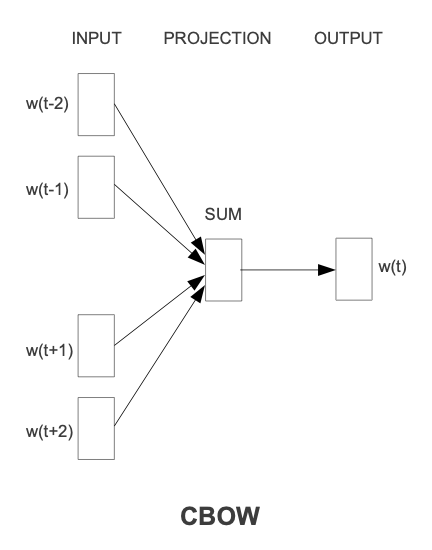
\includegraphics[width=0.4\textwidth]{../img/cbow.png}
	\caption{CBOW model \citep{mikolov2013efficient}.}
	\label{cbow}
\end{figure}
 \newpage
\subsection{(Distil)BERT for single sequence classification}

Transformer networks took the world by storm due to its paralellization capabilities and toppled established architectures such as LSTMs with new state of the art scores in several NLP tasks. While a traditional transformer has encoder and decoder blocks, Bidirectional Encoder Representation from Transformers (BERT), as the name suggests, only has encoder blocks \citep{halthor2020}. The BERT architecture is pre-trained with huge corpora such the BookCorpus (800M words) and English Wikipedia (2,500M words) \citep{devlin2019bert}.

BERT uses two techniques simultaneously for pre-training: Masked Language Model (MLM) and Next Sentence Prediction (NSP). The former consists into masking out a certain amount of words from sentences and training to predict those words, e.g. "The corona [MASK] outbreak" and the prediction of the word "virus". The latter is the task of judging if a sentence is a continuation of a previous sentence, e.g. The sentence "Voted in Nicaraguan elections" does \textit{not} follow the sentence "The penguins of Antartica." The first task is responsible to train context \textit{within} the sentence, while the second task trains context between sentences.

Every sequence in BERT has the special [CLS] token as the first token (see Figure~\ref{fig-cls}). Additionally, every BERT input embedding, $\mathit{E}$, is the sum of three different embeddings: token, segment, and position. The token embedding is retrieved from the pre-trained WordPiece embeddings, with a 30,000 token vocabulary. The segment embeddings encode which sequence it is dealing with (sequence A or B in a NSP task). Finally, the positional embedding is encodes a word's position in that sentence. This embedding \textit{E} is then fed into the network and the last hidden state of the [CLS] token can be seen as agregate sequence representation that can be used for classification \citep{devlin2019bert} as seen on Figure~\ref{fig-bert}.

\begin{figure}[!h]
	\centering
	\subfloat[]{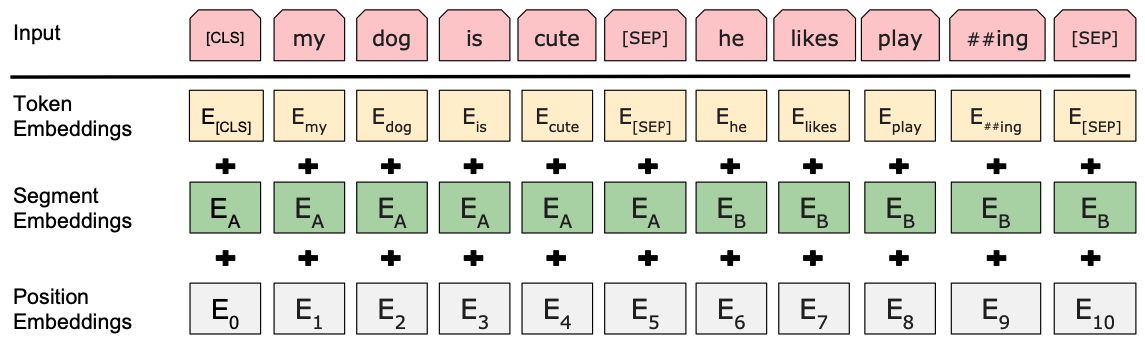
\includegraphics[width=0.6\textwidth]{../img/embeddings.png}\label{fig-cls}}
	\hfill
	\subfloat[]{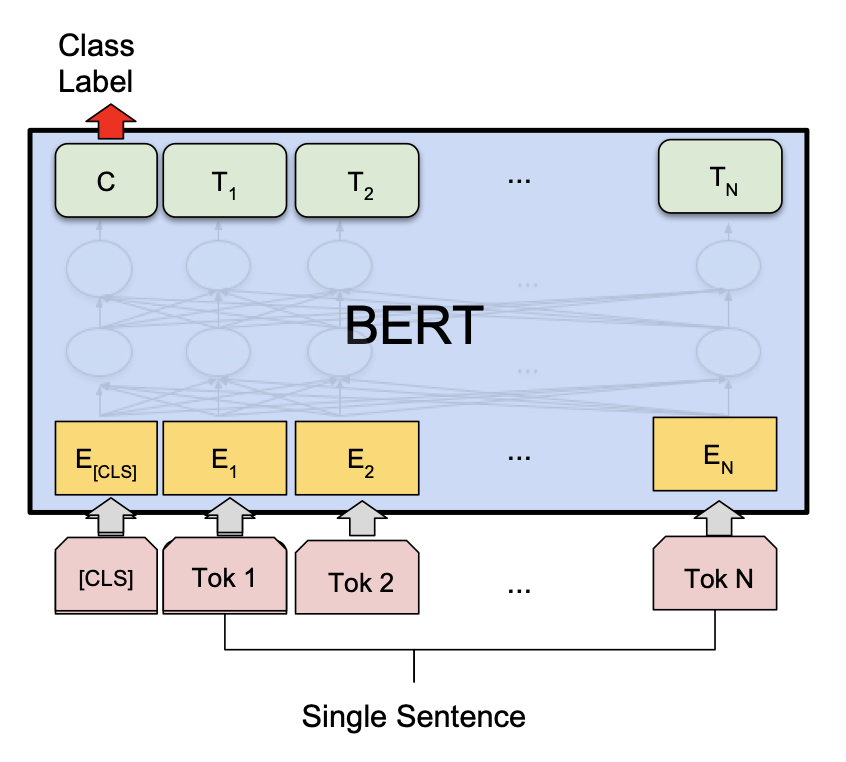
\includegraphics[width=0.4\textwidth]{../img/BERT-class.png}\label{fig-bert}}
	\caption{(a) BERT's input representation and (b) BERT for single sequence classification \citep{devlin2019bert}.}
\end{figure}



The distilBERT model is a case of transfer learning technique called distillation where a "student" model is trained to achieve  the behaviour of a larger "teacher" model \citep{sanh2020distilbert}. This managed to "reduce the size of a BERT model by 40\%, while retaining 97\% of its language understanding capabilities and being 60\% faster" \citep{sanh2020distilbert}.



\subsection{Linear Support Vector Classification}

Given pairs of observations -- word embeddings -- and labels -- sarcastic or not -- $(\mathbf{x}_i, y_i)$, a support vector classifier tries to find the hyperplane which maximizes the margins between classes \citep{pena2019}. The kernel used in classification can vary, but for NLP applications where the numbers of features are large, the linear kernel is more suitable given that text data is often linearly separable and the computations are faster \citep{hsu2003}. The prediction is given by Equation~\ref{eqn:svm} and  the maximum margin is given by Equation~\ref{eqn:margin} \citep{pena2019} 

\begin{equation}
	\label{eqn:svm}
 	\hat{y}= \mathbf{xw} +  b
\end{equation}

\begin{equation}
	\label{eqn:margin}
	argmax_{\mathbf{w}, b} \frac{1}{||\mathbf{w}||}
\end{equation}


	\newpage
	\thispagestyle{plain}

\section{Data}

The data used was  the \href{https://www.kaggle.com/rmisra/news-headlines-dataset-for-sarcasm-detection}{\color{blue}{News Headlines Dataset For Sarcasm Detection}}\citep{misra2019sarcasm} found on Kaggle.  This dataset consists of news headlines from two different websites: \href{https://www.theonion.com}{\color{blue}{The Onion}}, a satiric news website where all headlines and articles are sarcastic/humorous, and \href{https://www.huffpost.com}{\color{blue}{Huffpost}}, a real news website where its headlines are considered 'not sarcastic'. It is clear that there is a difference in tone and language when it comes to these websites, as evidenced in Figure~\ref{fig-huff} and~\ref{fig-onion}. 

\begin{figure}[!htb]
	\centering
	\subfloat[]{
\includegraphics[width=0.43\textwidth]{../img/huffpost.png}\label{fig-huff}}
	\hfill
	\subfloat[]{
\includegraphics[width=0.5\textwidth]{../img/the-onion.png}\label{fig-onion}}
	\caption{Sample of (a) not sarcastic and (b) sarcastic headlines from Huffpost and The Onion.}
\end{figure}

The raw data is in JSON format and contains information on 28619 headlines. The fields available are:

\begin{itemize}
	\itemsep0em 
	\item{is\_sarcastic: Boolean.Wheter the headline is sarcastic or not.}
	\item{headline: String. Headline text.}
	\item{article\_link: String. URL pointing to the headline's article.}
\end{itemize}

The analysis of this report is focused on the headline text and its class. The article link, therefore, is discarded. Apart from that, no further preprocessing was done.

The classes were found to be fairly balanced, as shown in Figure~\ref{counts} and ~\ref{freq}: 14985 non-sarcastic headlines against 13634 sarcastic ones, that is 52,36\% and 47,64\% of the total headlines respectively. A sample of the dataset is available in Table ~\ref{table:sample}.

\begin{figure}[!tbp]
	\centering
	\subfloat[]{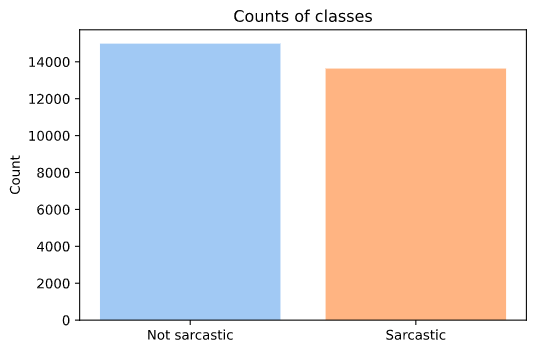
\includegraphics[width=0.5\textwidth]{../img/counts.png}\label{counts}}
	\hfill
	\subfloat[]{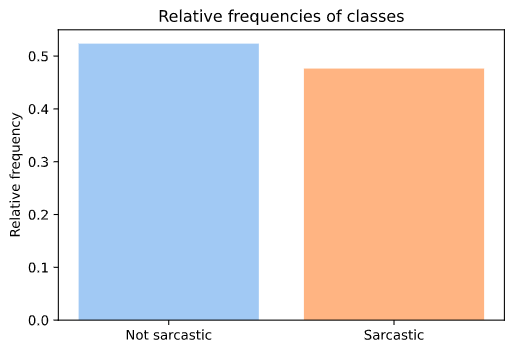
\includegraphics[width=0.48\textwidth]{../img/freq.png}\label{freq}}
	\label{class-balance}
	\caption{(a) Absolute count and (b) Relative frequencies of classes.}
\end{figure}

\newpage
\begin{longtable}[]{p{12cm}lp{}}
	\toprule
	Text & Label \tabularnewline
	\midrule
	\endhead
	'thirtysomething scientists unveil doomsday clock of hair loss'  & 1 \\ \tabularnewline
	
	'dem rep. totally nails why congress is falling short on gender, racial equality' & 0 \\ \tabularnewline
	
	'eat your veggies: 9 deliciously different recipes' & 0  \\ \tabularnewline
	
	'inclement weather prevents liar from getting to work' & 1\\   \tabularnewline
	
	"mother comes pretty close to using word 'streaming' correctly" & 1 \\ \tabularnewline
	
	'my white inheritance' & 0\\ \tabularnewline
	
	'5 ways to file your taxes with less stress' & 0 \\ \tabularnewline
	
	"richard branson's global-warming donation nearly as much as cost of failed balloon trips" & 1 \tabularnewline

	\bottomrule
	\caption{Sample of final dataset.}
	\label{table:sample}
\end{longtable}






	\newpage
	\thispagestyle{plain}

\section{Method}

In this section there will be details on how the study was carried, such as packages, pre-trained models and functions used. For all methods, the same training and test sets were used: 67\% of headlines were used for training and 33\% for testing. A fixed random seed of 42 ensures the reproducibility of results throughout the different methods. 

Stop word removal and lemmatization were initially tested, but yielded worse results than the raw text. For this reason, no special pre-processing of text was used.

All methods are made of some type of vectorization of text and then fed to a \code{LinearSVC} classifier. Accuracy, recall and F1 scores were computed using Scikit-Learn's  \code{classification\_report}. Additionally, the \code{plot\_confusion\_matrix} was used to visualize the results. For even more details on coding, the reader is referred to Section ~\ref{appendix} - Appendix.

\subsection{Baseline: Random chance}

The use of Scikit-Learn's \code{DummyClassifier} and \code{Pipeline} tools made this evaluation straightforward. The classifier was configured to the default stratified method, i.e. it will respect the class distribution (as stated previously, 52,36\% not sarcastic and 47,64\% sarcastic). After the instantiation of the pipeline, it was just a matter of fitting the classifier to training data and predicting on test data via the methods \code{pipeline.fit} and \code{pipeline.predict}.

\subsection{TF-IDF}

The key tool used in this section was Scikit-Learn's \code{TfidfVectorizer} function inside the pipeline. The \code{max\_features} and \code{ngram\_range} were set to 1000 and (1,2), respectively. The first parameter will only retrieve the top 1000 words in term frequency, while the second parameter will extract unigrams and bigrams from the corpus. After that, the classification routine proceeds as usual.

\subsection{Word2Vec - CBOW}

To extract Word2Vec embeddings, the spaCy library was used. The pre-trained pipeline \code{en\_core\_web\_lg} comes with built-in, 300 dimensional, word vectors. Every document (i.e. headline) was vectorized as the average of their token vectors \citep{spacy} and fed to the classifier.

 \subsection{DistilBERT}
 
 Pre-trained tokenizer and model were used in this section. More specifically, Hugging Face's \code{distilbert-base-uncased} model. The steps involved were adapted from \cite{alammar2019}.
 
 The tokenizer step preparess text to be fed to the distilBERT network. More importantly, it adds the special [CLS] (which has an id of [101]) token at the beginning of every sequence, which will be crucial to classification later on. Given the average word count in all headlines was around 10 words/headline and that the vast majority of headlines were 12 words or shorter as seen on Table~\ref{table:stats}, an embedding dimension of 25 was chosen as a good compromise between shorter and longer headlines. That way, shorter headlines will be padded with zeroes and longer headlines will be truncated. distilBERT's tokenizer not only tokenize words, but it will also split words into pieces (wordpiece tokenization).
 
 \begin{longtable}[]{p{5cm}lp{}}
 	\toprule
 	\centering Statistics & \centering Value \tabularnewline
 	\midrule
 	\endhead
 	Headlines & 28619 \tabularnewline
 	Average words per headline & 10.05 \tabularnewline
 	Standard deviation & 3.39  \tabularnewline
 	Min & 2 \tabularnewline
 	25\% & 8  \tabularnewline
 	50\% & 10 \tabularnewline
 	75\% & 12 \tabularnewline
 	Max & 151 \tabularnewline
 	
 	\bottomrule
 	\caption{Descriptive statistics of sentences.}
 	\label{table:stats}
 \end{longtable}
 
 
 An example of tokenization is as follows:
 
||A raw text headline: \code{thirtysomething scientists unveil doomsday clock of hair loss}

|| This is the (wordpiece) tokenized headline, padded: \code{['[CLS]', 'thirty', '\#\#some', '\#\#thing', 'scientists', 'un', '\#\#ve', '\#\#il', 'doom', '\#\#sd', '\#\#ay', 'clock', 'of', 'hair', 'loss', '[SEP]', '[PAD]', '[PAD]', '[PAD]', '[PAD]', '[PAD]', '[PAD]', '[PAD]', '[PAD]', '[PAD]']}
 
 ||This is the token ID headline, padded:  \code{[101, 4228, 14045, 20744, 6529, 4895, 3726, 4014, 12677, 16150, 4710, 5119, 1997, 2606, 3279, 102, 0, 0, 0, 0, 0, 0, 0, 0, 0]}
 
 The token id vectors were then fed to the distilBERT network. For every input (token id), 768 hidden units were outputted. The only hidden units of interest here are the ones tied to the [CLS] token. After slicing the output tensor to retrieve those units, they were then fed to the classifier.  
	\newpage
	\thispagestyle{plain}

\section{Results}

In addition to  classification accuracy, relative increase of this metric with respect to the previous one is displayed on Table~\ref{tableacc}. Random choice, as expected, performed worse with 50\% accuracy, followed by a significant increase with TF-IDF vectorization. CBOW embeddings slightly improved accuracy up to 81\%. DistilBERT embeddings achieve the highest accuracy, 86\%, a 6.2\% increase from CBOW and a 72\% increase relative to the dummy classifier. These results are also reflected in Figure~\ref{cm} where the confusion matrices for all methods are displayed.

\begin{table}[h]
	\centering
	\resizebox{7cm}{!}{%
		\begin{tabular}{lcc}
			\hline
			\multicolumn{1}{c}{Method} & Accuracy & Relative increase \\ \hline
			Random choice              & 0.5      & 0\%               \\ 
			TF-IDF                     & 0.79     & 58\%              \\ 
			CBOW                       & 0.81     & 2.5\%             \\ 
			distilBERT                 & 0.86     & 6.2\%             \\ \hline
		\end{tabular}%
	}
\caption{Accuracy for different vectorization/embeddings.}
\label{tableacc}
\end{table}



\begin{figure}[h]
	\begin{tabular}{cc}
		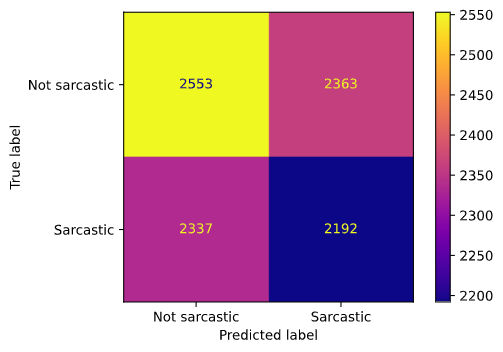
\includegraphics[width=70mm]{../img/dummy-cm.png}\label{cmrandom} &   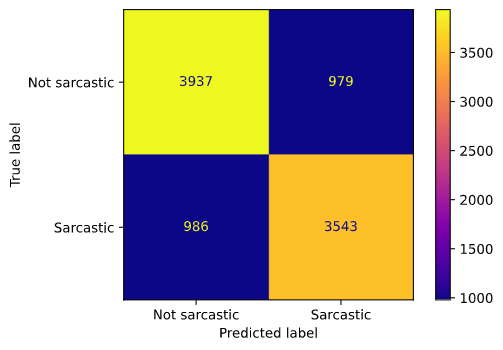
\includegraphics[width=70mm]{../img/tfidf-cm.png}\label{cmtfidf} \\
		(a) Random choice & (b) TF-IDF \\[6pt]
		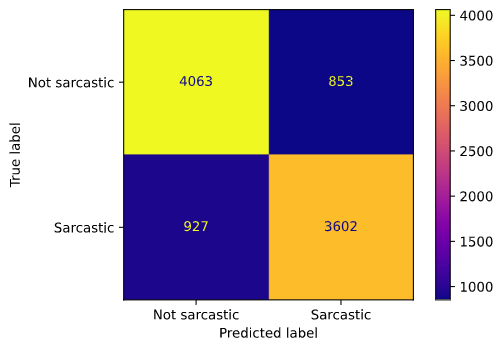
\includegraphics[width=70mm]{../img/w2v-cm.png}\label{cmcbow} &   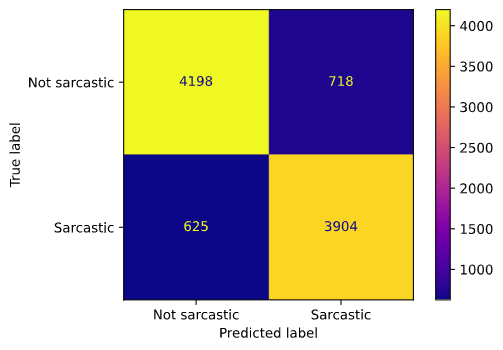
\includegraphics[width=70mm]{../img/bert-cm.png}\label{cmdistilbert} \\
		(c) CBOW & (d) distilBERT \\[6pt]
	\end{tabular}
	
	\caption{Confusion matrices}
	\label{cm}
\end{figure}
	\newpage
	\thispagestyle{plain}

\section{Discussion}

From the results of the previous section, it is evident that more powerful algorithms/models yield best classification results. This is specially the case for distilBERT, who achieved the highest accuracy of all tested methods. This can be explained by context capturing (via positional embeddings), which distilBERT does while the other methods do not. Still, CBOW achieved relatively good metrics. On the other hand, distilBERT was significantly more computationally heavy: this is considered a small dataset and even with a small 25 tokenized dimensions, the evaluation took almost an hour to train. Of course, the use of parallelization (which is highly recommended) was not used, which in itself could be an improvement for next projects/larger corpora.

One clear limitation of the work is in the data itself. The fact that a headline comes from a "serious" news website does not imply the absence of sarcasm. Sarcasm is a good communication tool to transmit opinion and is wildly used throughout media, serious or not. As an improvement, more traditional sarcasm datasets could be used to compare with previous work, such as the Twitter and/or Reddit corpus.

Another limitation was the somewhat simple conduction of experiments: a lot more could have been done in terms of hyperparameter tuning, both for the vectorization/embeddings and for the classifier. Some examples of this could be vocabulary size in TF-IDF, different tokenization dimensions, and number hidden layers/attention heads in distilBERT. Also other classifiers could have been used for comparison.

The biggest limitation, however, was that the distilBERT model was not fine-tuned for this task.  It is believed the even better accuracy could have been achieved with it. Nonetheless, the higher performance of transformer models in figurative language detection is not surprising, as evidenced in \citep{potamias2020}.
	\thispagestyle{plain}

\section{Conclusion}

While this project had its limitations, it was possible to see that indeed transformer networks such as distilBERT are more suitable for highly context-dependent NLP tasks such as sarcasm detection. The power of transfomers comes with a caveat: these models are significantly more computationally demanding and need to use parallelization to be efficient. The results could be improved via a more optimized dataset and fine-tuning.

In conclusion, a not-so-black-box view of this project allowed for an initial contact with the transformer architecture, its power, and its importance to the NLP world.
	\section{Appendix: Code and data} \label{appendix}
	
	The preprocessed data and code used in the making of this report can be found in this \href{https://github.com/cosmourao/sarcasm-tm}{\color{blue}{repository}}.
	\bibliography{references}
	\bibliographystyle{apalike}
\end{document}


